\chapter{内侧前额叶皮层:基于输出结果选择动作} \label{chap:chap3}

这本书提出了关于灵长类动物前额叶皮层基本功能的方案。



\section{概述}
内侧前额叶皮层有助于评估和选择基于先前行为结果的行为,其连接指纹解释了它是如何做到这一点的。
海马连接提供有关导航和其他涉及行动事件的信息,杏仁核提供基于当前生物需求的预测结果的最新评估,并且与内侧前运动区域的连接提供了行动的途径。
这些涉及行为和动机的“内部”信号与外部信号(如感官输入)形成对比。
内侧前额叶皮层基于这些内部因素对行动的选择产生偏见,包括努力成本、更新估值、预测结果对觅食选择的影响,以及使用内在与外在坐标系来指导行动。
在灵长类动物中,内侧前额叶皮层的颗粒部分通过在反馈时间评估自我产生的选择、平衡竞争性任务规则以及根据单个先前事件做出选择来阐述这些“内部”影响。\par



\section{介绍}

第一章解释了连接限制了前额叶皮层的功能。
由于其连接因区域而异,本章开始对前额叶皮层进行区域探索。
我们从内侧前额叶皮层开始,部分原因是它包括前额叶皮层的一些较老部分(第二章)。\par

第\ref{chap:chap2}章区分了内侧前额叶皮层的颗粒状部分和无颗粒状部分,后者在所有哺乳动物中都有。
因此,我们想比较大鼠和猴子的无颗粒状前额叶皮层。
不幸的是,对猴子的这些区域知之甚少。
因此,我们被迫依赖啮齿动物(主要是大鼠)的数据。
我们认识到这种方法的危险 - 啮齿动物和灵长类动物的最后共同祖先生活在大约70-90 Ma,从那以后这两个谱系就分开进化了。
这一事实意味着,随着两组动物的进化,两组动物的无颗粒状前额叶区域的连接和功能将发生变化。
未来的研究将表明这种差异的程度,但现在我们必须利用我们所拥有的东西来研究。\par


在灵长类动物中,内侧前额叶皮层位于内侧前运动区域的喙部,包括前SMA,SMA和CMA(见缩写列表)。
Passingham等\cite{passingham2010medial}认为,所有这些中间领域都显示出指导和分析基于“内部”信号的行动的专业化。
“内部”一词,在这里使用的意义上,是指传达内部状态和记忆的信号,与视觉、听觉、嗅觉、味觉和触觉等外部信号形成鲜明对比。



\section{区域}

图\ref{fig:3_1}显示了猴子和人类中被指定为内侧前额叶皮层的区域,图\ref{fig:fig_2_1}显示了其在猴子,人类和大鼠中的细分视图。
在灵长类动物中,内侧前额叶皮层的颗粒部分由前扣带皮层(区域24),边缘前皮层(主要是区域32)和边缘下皮层(区域25)组成。
正如第\ref{chap:chap2}章所解释的,所有哺乳动物,包括啮齿动物和灵长类动物,都有这三个区域的同系物。\par
内侧前额叶皮层的颗粒部分包括区域9的内侧部分和所有区域10,只有灵长类动物有这些区域。
第\ref{chap:chap1}章证明将极地包括在内是合理的前额叶皮层(区域10)在内侧区域组,部分基于连接。
注意我们将所有额极皮层(区域10)都包括在周一的内侧前额叶皮层内键,但只是它在人类中的内侧部分。


\begin{figure}[!htb]
	\centering
	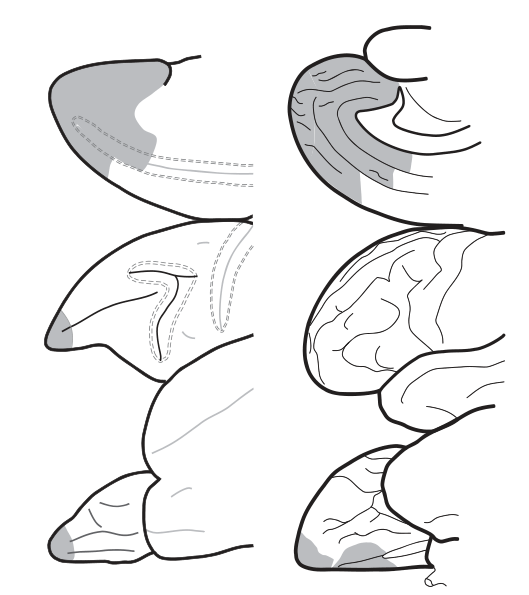
\includegraphics{image_pfc/Fig_3_1}
	\caption{猕猴(左)和人类(右)的内侧前额叶皮层,用阴影表示。格式如图\ref{fig:1_2}所示。}
	\label{fig:3_1}
\end{figure}


术语前扣带皮层在文献中有很多含义。
在这本书中,我们将边缘前皮层和边缘下皮层排除在我们称为前扣带皮层(图\ref{fig:fig_2_1})。
我们还排除了扣带运动区域,这些区域我们认为是前运动皮层的一部分。
因此,读者应该意识到当我们使用短语前扣带皮层,我们仅指区域 24 的一部分,而不是到运动前区域或内侧前额叶皮层的其他颗粒状部分。\par


在我们排除在前扣带皮层之外的区域中,眶前和边缘下皮层占据了大部分的眶前和眶下皮层。
术语膝下皮层是指胼胝体膝腹侧的皮层,术语膝前皮层是指位于膝侧的无核区域。
孕皮质不包括位于更前列的颗粒区域,例如额极皮层的内侧部分(区域10)。
最后,我们称之为腹内侧前额叶皮层的14区的状态仍不确定。
一些专家将其纳入内侧前额叶皮层,另一些专家则将其视为眶额皮层的最内侧部分。
我们不需要在这些分类之间做出决定,但在大多数情况下,我们保留了第\ref{chap:chap4}章关于眶额皮层的区域14的考虑。\par



\section{连接}

图\ref{fig:3_2}显示了猕猴内侧前额叶皮层的主要连接。
这个情节和第\ref{chap:chap4}-\ref{chap:chap7}章中的类似情节旨在传达神经解剖学文献中出现的最重要的概念点。
我们不打算提供一个全面的总结,也不关心指出哪些神经解剖学家首先描述了一个特定的途径。
这些情节起到了连接指纹的作用,第\ref{chap:chap1}章对此进行了解释。
连接指纹强调区分前额叶皮层区域彼此和其他皮层区域的特征,就像人类指纹区分人与人一样。\par


1.海马体和下托与内侧前额叶皮层的边缘下和边缘前区域有密集的相互连接\cite{insausti2001cortical}。
海马体和内侧前额叶皮层之间的间接连接包括前扣带皮层(区域24)和内侧颗粒区域9和10,其中一些通过脾后皮层运行\cite{kobayashi2003macaque}。
内嗅皮层和海马旁皮层也与内侧前额叶皮层有联系\cite{kondo2003differential,munoz2005cortical}。
海马体和内侧前额叶皮层之间的皮质下通路包括通过乳头体和丘脑的中继。
我们认为与海马体的联系对内侧前额叶皮层的功能特别重要。其他前额叶皮层区域,如外侧眶额皮层,要么缺乏与海马体的连接,要么具有非常弱的连接\cite{carmichael1995limbic}。
稍后,我们解释了我们的观点,即海马体为前额叶皮层提供了有关导航和其他涉及动作的过去事件的信息。


2.内侧前额叶皮层与杏仁核有着紧密的联系,图\ref{fig:3_3}显示,这些投射中密度最大的涉及前额叶皮层的无核部分\par


\begin{figure}[!htb]
	\centering
	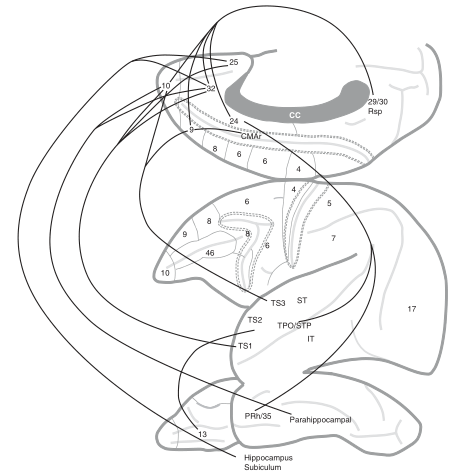
\includegraphics{image_pfc/Fig_3_2}
	\caption{猕猴内侧前额叶皮层的选定连接。
		图\ref{fig:1_4}和\ref{fig:1_5}给出了沟和区域的名称。
		线连接着一些有直接轴突连接的区域,除非另有说明,否则假设是相互的。}
	\label{fig:3_2}
\end{figure}


\cite{prather2001increased,morecraft2007amygdala}颗粒区域,如13m区域,也接受杏仁核输入,图\ref{fig:3_3}没有说明\cite{saleem2008complementary}\par
杏仁核通常被视为在情绪、动机和奖励中发挥作用,包括恐惧调节和对社会刺激(如人脸)的情绪反应。
但它在奖励中的作用并不是一般的。
双侧杏仁核损伤后,条件性视运动学习完全正常进行,尽管这取决于学习与奖励的关系\cite{murray1996role}。
因此,奖赏处理本身不能作为杏仁核功能的一般或完整描述。
相反,最有力的证据表明,杏仁核和皮层之间的相互作用会根据当前的需求更新结果评估\cite{baxter2002amygdala}。
在整本书中,我们使用结果一词来指代以下反馈\par


\begin{figure}[!htb]
	\centering
	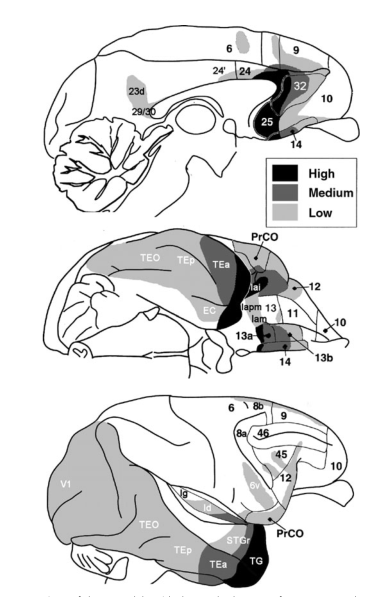
\includegraphics{image_pfc/Fig_3_3}
	\caption{猕猴杏仁核与大脑皮层的连接。
		阴影表示投射的主观密度,重点是从杏仁核到皮层的投射。
		皮层通常也会发送一个返回投影。
		缩写:EC,内嗅皮层;Iai、Iapm和Iam,分别为无核岛状区、下分区、后内侧分区和内侧分区;Ig,颗粒状岛叶皮层;Id,粒状岛叶皮层;中央前顶盖皮质;颞上回;TEa、TEp、TEO、颞下区、前部、后部和枕部;TG,颞极皮层;V1,初级视觉(纹状体)皮层(17区)。
		经麦克米伦出版有限公司(Macmillan Publishers Ltd.)普莱斯·JL(Price JL)、德雷维茨·WC(Drevets WC)许可转载。《情绪障碍的神经回路》,《神经精神药理学》35:192–216,©2009,自然出版集团}
	\label{fig:3_3}
\end{figure}


一种行动,无论是从发生的事情还是在任何特定时间的价值来看。
当然,目前的需求不仅涉及营养和液体,还涉及避免伤害和其他生物成本和收益。
因此,我们可以说杏仁核有助于评估积极和消极的结果。\par


3.内侧前额叶皮层直接或间接投射到运动前区域。
颗粒内侧前额叶皮层(9区)与内侧前额叶皮层的其他部分有联系,特别是与前扣带皮层有联系\cite{vogt1987cingulate}。
该区域反过来与前扣带运动区(CMAr)相连,CMAr是内侧前运动皮层的一部分\cite{morecraft1998convergence}。
CMAr位于扣带沟\cite{dum2002motor},位于与之相连的术前运动区(preSMA)的腹侧\cite{luppino1993corticocortical}。
SMA本身也与尾扣带运动区相互连接\cite{luppino1993corticocortical}。
扣带运动区或前SMA和SMA的损伤损害了猴子在没有外部(感觉)提示的情况下做出的运动的产生\cite{thaler1995functions}。
因此,我们可以将这些行动称为“内部”指导\par


4.与腹侧前额叶皮层和眶侧前额叶皮层不同,内侧前额叶皮层不接收来自颞下皮层的视觉输入\cite{carmichael1995sensory,kondo2005differential}。
然而,前扣带皮层与嗅周皮层有一些联系,它也接收来自颞上沟TPO区域的输入\cite{kondo2005differential},该区域处理视觉和听觉信息。尽管有这些输入,内侧前额叶皮层和视觉区域之间的联系并不是特别突出。\par


5.内侧前额叶皮层,尤其是额极皮层(区域10),接收来自颞上皮层的投射,其中大部分来自其吻部,包括颞极\cite{barbas1999medial,kondo2003differential}\par
这些投射中一些更尾部的涉及生理学研究表明是听觉的区域\cite{hackett1998subdivisions},但其他投射的功能,如靠近颞极的投射,仍然未知\par


6.与前额叶皮层的许多其他部分不同,内侧前额叶皮层也投射到下丘脑\cite{rempel1998topographic},以及在内脏运动功能中发挥作用的脑干网状核\cite{ongur1998prefrontal}\par


其中一些投射可能会影响自主神经系统,以及大脑控制身体的其他方式。
例如,下丘脑外侧调节自主神经的唤醒,下丘脑的室旁核控制神经内分泌和神经分泌的输出。\par



\subsection{总结}

内侧前额叶皮层的连接指纹表明以下要点:
(1)与前额叶皮层的其他部分相比,内侧前额叶皮层接收的感觉输入很少;
(2) 它与运动前区域相连,该运动前区域在动物蓄能器网络71缺乏来自任何外部线索的动作提示时控制动作;
(3)它与海马体和杏仁核有着密切的联系,这表明它既可以获得过去事件的记忆,也可以获得从当前生物需求来看有价值的结果信息\par


尽管这里列出的连接并不总是涉及内侧前额叶皮层的相同部分,但不同部分相互连接\cite{barbas2000connections},这意味着一个部分的输入可以影响其他部分。
第\ref{chap:chap8}章将这一观点扩展到整个前额叶皮层。\par



\section{决策、选择和目标}

尽管“决定”一词可以应用于动物所做的大多数事情,但我们使用这个词的方式更为有限。
我们将决策与这些决策之后可能做出的选择和采取的行动区分开来\cite{schall2001neural}。
决策涉及基于感官输入的感知。
从这个意义上说,决定并不是直接指动物所做的任何事情。
因此,动物会做出感性的决定,而不是感性的选择。
它们做出觅食的选择,而不是觅食的决定\par


作为其决策的结果,动物可能会选择一个目标,并基于这个目标的选择,它可能会选择行动。
或者,动物可以直接在动作中进行选择。在整本书中,我们使用目标一词来指代动物选择作为其行动目标的物体或位置。
然后,这一行动产生了一个结果,包括动物所获得的利益或因其行为而产生的成本。
因此,我们将目标与结果区分开来,从不将目标一词用作结果的同义词。\par


我们知道,在文献中,使用目标一词来表示动物在行为实验中获得的奖励是很常见的。
事实上,在这些实验中,奖励是动物的最终目标。
但为了获得奖励,动物通常必须选择一个物体或地点作为其行动的目标。
因此,我们为这些对象和地点保留目标,并始终使用结果来奖励和其他形式的行动或事件反馈。
这个术语有助于本书中许多地方的讨论,读者需要记住我们使用这些术语的方式,以及它与文献中其他使用的不同之处\par


我们还区分了基于外部或“内部”线索的选择\cite{Passingham et al.2010}。
例如,猴子可以使用远处的视觉标志来选择觅食目标,比如远处树上的水果或树叶。
因此,它们根据外部的感官信号产生一个目标——水果或树叶。
但猴子也可以根据它们的记忆或内部状态的变化(如饥饿)来产生目标。
由于没有更好的词,我们说在这种情况下,动物是根据“内部”信号行事的。
稍后,我们将讨论内侧前额叶皮层在外部和“内部”信号竞争时的作用\par



\section{累加器网络}

累加器-赛道模型为这种神经竞争提供了一种机制,因此我们在这里给出了一个非常简短的描述。
尽管累加器网络已经了解这些模型将使读者更容易理解对内侧前额叶皮层的输入如何导致动作,以及来自内侧前额叶皮质的输出如何会使其他类似网络产生偏见。
在本章的后面,我们将看到这些想法在内侧前额叶皮层的功能中的具体应用,这些功能可以做出与觅食类似的选择\par


猴子的神经生理学实验说明了累加器网络是如何工作的。
当神经网络达到产生输出的阈值时,就会做出决策、选择和行动。
这些网络就像漏洞百出的积分器,积累有利于其输出的“证据”:网络所代表的决策、选择或行动。
一旦它们达到阈值,网络的输出就会引起一系列影响,这些影响可能最终导致电机命令的执行,要么通过驱动电机模式发生器的活动,要么将其从紧张抑制中释放出来。
各种类型的累加器网络并行运行,因此可以说是相互竞争\par


图\ref{fig:3_4}显示了一个弹出实验的结果。
在这类实验中,猴子的视野中会出现许多刺激物。
它们大多数都有相同的特征,如颜色和形状,但有一个不同。
在得出图\ref{fig:3_4}的实验中,猴子看到了七个红色方块和一个绿色方块,这八个刺激物在以注视点为中心的圆的圆周上等距出现。
为了在每次试验中获得奖励,猴子必须做一个扫视的眼球运动来固定绿色的正方形。
与所有任务一样,从八种刺激出现到猴子开始运动的时间(称为反应时间)因试验而异,但通常在175-225毫秒之间。
在第\ref{chap:chap5}章中,这个实验涉及眼球运动这一事实变得很重要,但就目前而言,运动的种类无关紧要。\par


\begin{figure}[!htb]
	\centering
	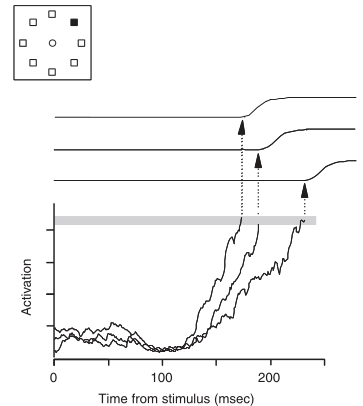
\includegraphics{image_pfc/Fig_3_4}
	\caption{额视野中的神经元活动。
		放电速率是刺激开始后时间的函数。
		随着活动的增加,它达到了扫视眼球运动的阈值(阴影水平条)。
		试验根据反应延迟分为三部分。
		左上角的插图显示了猴子观察到的显示,其中一个刺激因其不同的颜色(黑色方块)而从八个刺激中“弹出”。
		转载自Schall JD,Thompson KG。视觉引导眼球运动的神经选择和控制。神经科学年度评论22:241–59©1999年年度评论,以经许可}
	\label{fig:3_4}
\end{figure}


累加器模型假设一些累加器集成了绿色刺激的证据。
可以说,这些累加器体现了一个“假设”,即刺激是绿色的,其输入是支持和反对这一假设的证据。
在单细胞水平上,信息的积累表现为上升的活动,直到达到阈值,有时称为爬升活动。
图\ref{fig:3_4}显示了这种攀爬活动,分为三组试验,根据猴子的反应时间进行排序。
在最短的反应时间内,细胞上升到由水平灰色条指定的给定水平,然后扫视很快开始。
没有直接证据表明这类神经元的整个网络在那一刻达到了阈值,但我们认为是这样。
如图所示,活性增加的速率越慢,反应时间越长\par


竞争的产生是因为这些神经网络的架构及其相互作用。
首先达到阈值的网络“赢得”比赛,它控制着它所代表的决策、选择或行动。
总的来说,这些回路以赢者通吃的方式工作,这反映了一个事实,即动物不能同时移动两个相反的方向,同样,在大多数情况下,也不会同时做出相互矛盾的决定和选择。\par


猴子必须辨别相干运动方向的实验说明了累加器网络的竞争方式。
在这项任务中,许多光点以相同的速度向同一方向移动,而其他光点则随机移动。
随着观看时间的延长和更多的光点向同一方向移动,决策的准确性会提高\cite{schall2001neural}已经回顾了这些神经元机制的证据。
根据他们的分析,几个区域的细胞增加了它们的活动,直到它们达到阈值:MT和MST区域的网络代表决策,LIP区域的网络表示选择,而FEF区域的网络则代表行动\cite{kim1999neural}。\par


图\ref{fig:3_5}显示了自上而下的有偏见的竞争是如何运作的。
在这种情况下,实验者在MT区域使用皮质内微刺激来模拟自上而下的信号。
以一个整合了向上运动证据的网络为例。
通过刺激网络中的神经元,它比没有微刺激的情况下更快地达到阈值。
这种人为的输入使“向上”的累加器更有可能赢得“比赛”,并做出圆点向上移动的决定。\par


活动上升到网络阈值,从而产生决策、选择或行动的速度取决于证据的强度和整合证据的可用时间。
它还取决于竞争累加器的活动,这些累加器为替代决策、选择和行动收集证据。\par


\begin{figure}[!htb]
	\centering
	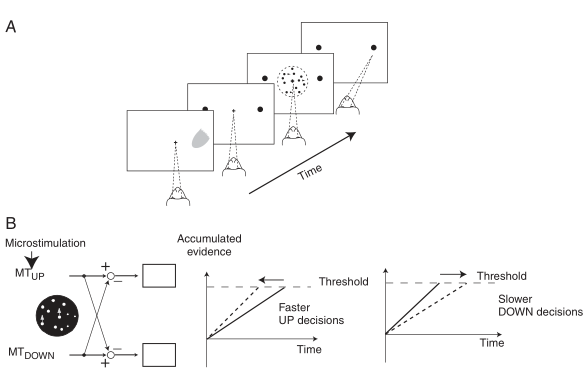
\includegraphics{image_pfc/Fig_3_5}
	\caption*{自上而下注意力的神经机制。
		(A) 猴子观察斑点,并在左右扫视目标之间进行选择,以报告斑点运动的方向。
		虚线在固定点处汇合。
		(B) 一些累加器网络集成了点向上移动的证据,另一些则集成了点向下移动的证据。
		当点向上移动时,由于皮质内微刺激,网络中的更大活动会导致其更快地达到“向上”决策的阈值,而“向下”决策的速度较慢(虚线)。
		缩写:MT UP,位于颞中区的细胞编码向上的斑点运动;MT DOWN,编码向下运动的细胞。+,兴奋性突触输入,抑制性输入。虚线显示皮质内微刺激期间的活动率;实线显示了在这种刺激之前和之后的活动。
		(A) 复制自Roitman JD,Shadlen MN。在组合视觉辨别反应时间任务中,顶内外侧区域神经元的反应。《神经科学杂志》22:9475–89©神经科学学会,2002年,经许可。
		(B) 转载自Ditterich J,Mazurek ME,Shadlen MN。视觉皮层的微刺激会影响感知决策的速度。《自然神经科学》6:891-8©2003。}
	\label{fig:3_5}
\end{figure}


作为“种族”的一个重要方面,积累矛盾证据的细胞可以相互抑制,如图\ref{fig:3_5}所示。
其他因素也会影响每个“种族”,包括每个网络的阈值、其兴奋性水平,以及推翻或否决决定、选择或行动的信号。
总之,这些网络中的许多网络之间的相互作用允许层次更高的网络对低阶网络产生的结果产生偏见。
对于内侧前额叶皮层,这涉及到与海马体、杏仁核、运动前皮层、下丘脑、中脑导水管周围灰质和其他结构的相互作用\par


在后面的章节中,我们认为前额叶皮层的其他区域也会对低阶区域发生的竞争产生偏见。
例如,第\ref{chap:chap5}章提供的证据表明,尾侧前额叶皮层可以对视觉区域施加自上而下的偏见,以增强对运动或形状的处理,这取决于它们与手头任务的相关性。
同样地第\ref{chap:chap8}章认为,当任务需要对行为进行集中控制时,前额叶皮层作为一个整体会产生自上而下的影响。\par



\subsection{总结}

像单电池一样,累加器网络集成输入,当它们达到阈值时,就会产生输出。
这些模型在证据和表征方面为决策、选择和行动提供了一种看似合理的神经元机制,而不仅仅是“祖母细胞”概念所体现的输入和发射。\par


为了总结本章的内容,内侧前额叶皮层有一组独特的连接,其特征是缺乏感觉输入,与海马体、杏仁核和内侧前运动皮层的相互作用密切。
其中一些连接驱动内侧前额叶皮层中的网络,一些连接将内侧前额叶皮层的输出传递到大脑的其他部分,在那里它们提供自上而下的偏置。
在下一节中,我们提出了一些证据,证明内侧前额叶皮层的无核部分偏向于竞争控制行为的低阶系统之间的竞争。\par



\section{啮齿动物的颗粒状皮层}

Murray等人\cite{murray2011can}提出,通过偏置争夺控制行为的大脑系统之间的竞争,内侧前额叶皮层可以在不直接产生运动命令的情况下影响动物的动作。
这个想法解释了哺乳动物的祖先在没有内侧前额叶皮层的情况下是如何相处得如此融洽的。
在没有这些领域的情况下,相互竞争的系统之间的联系最强。这种力量平衡可以改变,但只能慢慢改变。
当它在早期哺乳动物中进化时,无核前额叶皮层提供了一种自上而下的偏见,促进了更快的变化,而不是一种全新的变化能力。
后来,特别是在第 \ref{chap:chap8} 章和第 \ref{chap:chap9} 章中,我们提出这种进步——更快的变化,更少的错误——在前额叶皮层的进化过程中反复发生,第 \ref{chap:chap5} 章对自上而下的偏见竞争进行了更一般的处理。\par


脊椎动物的许多行为都依赖于系统发育上古老的强化学习机制。
其中包括古典(巴甫洛夫)和工具(操作)条件反射\cite{Dickinson 1980}。
在传统的动物学习理论中,奖励会加强存在时活跃的联想,这一过程被称为强化。
通过这种强化学习机制,刺激、反应和结果的表征之间会产生关联。每个表示可以链接到其他表示,并且它们可以分别缩写为S、R和O。
在经典条件反射中,刺激S与结果O相关联,可以称之为S–O映射。
在仪器条件作用中,反应R与结果O相关联,称为R–O映射。
在后一种情况下,这种关联可能发生在特定的刺激上下文S中,从而产生S–R–O映射。
“反应”和“行动”这两个术语的含义差别不大。
前者通常意味着存在一种启动刺激,而后者则不需要。
我们不时使用S–R、R–O等的紧凑表示法,而不区分动作和响应\par


在动物获得了特定的S–R–O和R–O关联的丰富经验后,它们的行为失去了对结果的依赖,并成为一种习惯。
程序性记忆一词有时用来指习惯,与陈述性记忆形成对比。我们避免使用这些术语,因为陈述性记忆的概念通常意味着意识,而我们不能谈论非人类动物的类人意识。\par


\cite{balleine2003effect}使用了一个简单的程序来区分结果导向动作和习惯动作。
实验人员可以操作性地调节动物执行给定的动作,从而产生一种奖励结果。
他们还可以让同一只动物进行第二次动作,从而产生第二种奖励结果。
一般来说,受试者发现这两种奖励都是可取的,尽管他们通常有偏好。
接下来,受试者有机会消费两种奖励中的一种,通常是饱腹感。消费这种奖励会使其相对于其他选择贬值。
在以后的测试中,被称为测试阶段,受试者可以在这两个动作之间做出选择。
除非他们养成了某种习惯,否则受试者将把大部分时间花在工作上,以获得最有价值的回报,这是根据他们当前的需求来评估的。
这意味着他们会避免产生最近消耗的奖励的行为。
因此,对其中一个奖励的讽刺会影响他们的行动选择。\par


大多数心理学家将这种性质的行为称为目标导向行为。
但正如我们已经提到的,我们保留目标一词来指行动的目标。
因此,我们将这些行为称为结果导向行为。\par


这些实验的一个重要特征是,动物在测试阶段接受任何奖励结果之前选择自己的行动。
也就是说,他们不需要在目前的饱腹状态下体验贬值的食物。
相反,受试者预测他们的行为将产生的奖励的价值,并据此做出选择。\par


在动物在这类任务上获得了如此多的经验,以至于养成了习惯之后,对其中一种奖励的满足感就不再影响它的行动。
动物继续选择在最近的一段时间内导致特定结果的行为,通常是首选食物,尽管这种结果已经贬值。
习惯也被称为S–R关联,因为动物在没有参考预测结果的情况下选择行动。养成一个习惯所需的训练量被称为过度训练。\par


请注意,一些专家用“习惯”一词来指代动物经常做的事情,或者人们不需要思考就能做的事情。
所以读者需要知道,我们并不是用这种宽泛的方式来使用习惯。\par


前面,我们解释了蓄能器-跑道模型的基本原理。
现在我们可以把这些原则应用到过度训练的动物习惯的产生上。根据累加器-跑道模型,一旦S-R关联足够强,它们的累加器网络总是在其他竞争网络到达阈值之前达到阈值,习惯就会占上风。
例如,假设S-R网络与S-R - o网络竞争。
我们认为,随着S-R网络连接的加强,它们将更快地达到阈值。
当这个过程达到没有其他网络可能“赢得”竞争的地步时,一个习惯就已经形成了。
在啮齿类动物77关联中,当一种粒状皮质支配其他粒状皮质时,可称为“优势”,而“优势行为”、“优势反应”、“优势行动”等短语都指的是这种概念。
这些术语既适用于先天行为,也适用于通过丰富的经验灌输的行为。优势行为在相对稳定的环境中提供了优势。\par


然而,对优势行为的依赖有代价也有好处。
它们的缺点是动物适应新环境的速度相对较慢。
在一个经典的例子中,绿蜥蜴(Lacerta)天生倾向于接近绿色,因为这能引导它们接近提供伪装和捕捉猎物机会的树叶。
Wagner\cite{wagner1932farbensinn}试图教这些蜥蜴在与理想食物相关的红色刺激和与掺假食物相关的绿色刺激之间做出选择。
为了训练蜥蜴选择红色刺激,科学家进行了数百次试验,尽管有些蜥蜴能轻易地区分红色和绿色,但它们还是做不到。
蜥蜴的优越行为在它们通常的生态环境中能很好的发挥作用,但因此它们无法灵活适应动荡的环境。\par


然而哺乳动物可以相对较快地学会这项任务。\cite{murray2011can}提供了非哺乳动物脊椎动物行为不灵活的其他例子,与哺乳动物的灵活性形成对比。
例如,老鼠可以学习位置任务的匹配。
在这项任务中,老鼠必须学会回到它们刚刚得到食物的地方\cite{marighetto1998effects}。
为了成功地完成这项任务,老鼠必须克服一种天生的倾向,即探索它们最近没有利用过的觅食地点,并避开那些它们已经利用过的地点。
完整的大鼠可以在15-20次训练中学习这项任务,但在内侧前额叶皮层的边缘前和边缘下区域受损后,大鼠的学习速度要慢得多\cite{dias2000effects}。
因此,与缺乏这些区域的动物相比,内侧前额叶皮层似乎赋予了更快、更少错误地从优势行为转变的能力。\par


另一项观察结果强化了这样一种观点,即病变大鼠无法轻易克服其天生的倾向:同样的病变大鼠可以以大约正常的速度学习不匹配定位任务\cite{dias2000effects}。
在这项任务中,动物必须避开刚收到食物的地方,选择迷宫的另一个分支。
因此,老鼠不必克服它们避开最近被开发的觅食地点的优越倾向。
这些想法解释了为什么患有边缘前和边缘下皮层病变的大鼠可以以正常的速度学习非匹配定位任务,但以异常缓慢的速度学习高度相似的匹配定位任务。\par


在野外,不同觅食地点的趋势在许多情况下都提供了优势。
耗尽的食物来源几乎没有什么好处。
然而,在某些情况下,例如当资源异常迅速地补充时,优势在于动物能够了解这种更新可能发生的背景,并能够抑制在其他地方寻找食物的优越倾向。
通过这种方式,皮层下大脑系统的上下偏置可以增强觅食选择的灵活性,而内侧前额叶皮层似乎在哺乳动物中提供了这种能力。
表3.1列出了动物在选择动作时面临的一些问题,以及内侧前额叶皮层可能带来的一些优势。\par


\begin{table}[htbp]
	\newcommand{\tabincell}[2]{\begin{tabular}{@{}#1@{}}#2\end{tabular}} %换行指令
	\centering
	\caption{选择行动的基本问题}
	\renewcommand\arraystretch{1.5}	%设置表格内行间距
	\begin{tabular}{c c }	 % 双竖线
		\hline	% 表格横线
		问题 & 解决方案 \\	
		\hline  % 横线
		不同的行动在回报和努力方面产生不同的结果 & 基于习得动作-结果关联的偏倚觅食选择 \\
		\hline
		动作可以基于外在坐标也可以基于内在坐标 & 偏向于那些基于外在或内在规则的觅食选择 \\
		\hline
		动作可以发生在稳定或易失的环境中 & 分别偏向那些基于习惯或基于预测结果的觅食选择 \\
		\hline
	\end{tabular}%
\end{table}%



\subsection{前边缘皮层和结果导向行为}

在大鼠中,内侧前额叶皮层包括三个区域,即前扣带皮层、边缘前皮层和边缘下皮层(见图\ref{fig:fig_2_1})。
正如我们已经提到的,位置匹配和不匹配任务的结果有助于阐明边缘前皮层的作用,但不能区分它们。
然而,有几项研究试图这样做。\par


当结果值发生变化时,脊髓前皮质的损伤会损害大鼠改变其行为的能力。
上一节描述的贬值测试揭示了动物根据当前需求调整选择的能力。
大脑皮质前病变的大鼠继续做出反应,产生高度贬值的奖励。
因此,前大脑皮层的损伤导致习惯性行为占主导地位,而非外向性行为\cite{balleine1998goal,corbit2003role}。
因此,我们可以得出结论,在正常大鼠中,前大脑皮层会根据结果导向的行为而不是习惯产生对觅食选择的偏见。\par


学习后发生的吸收前皮层损伤没有这种影响\cite{ostlund2005lesions},这也与该区域产生对结果导向行为的偏见的观点一致。
S–R联想(习惯)与S–R–O联想同时发展。经过广泛的经验,习惯可以控制行为,因此前大脑皮层的影响变得不那么重要了。\par


边缘下皮质似乎提供了相反的偏见。
Killcross\cite{killcross2003coordination}发现,边缘前皮质和边缘下皮质的作用存在双重分离。
他们证实了刚刚提到的这一发现,即大脑前皮层的损伤使大鼠对实验操作的当前奖励值不敏感。
边缘下皮质的病变没有这种影响。在这些损伤之后,即使经过了通常会产生习惯性行为的漫长过度训练期,大鼠的选择仍然会受到当前奖励值的影响。
因此,我们可以得出结论,在正常大鼠中,边缘下皮层提供了对习惯的偏见。
如果没有这种偏见,即使在预期习惯的情况下,行为仍然是以结果为导向的。\par


这些发现表明了这些区域在正常大鼠中所起的作用:边缘前皮层基于S–R–O关联(结果导向的行为)使行为偏向于觅食选择,而边缘下皮层则对同时发生的行为产生偏见学会了S–R联想(习惯)。
更广泛地说,这些领域似乎影响了S–R–O和S–R协会之间对行动选择控制权的竞争。\par


如果是这样,为什么内侧前额叶皮层需要两个区域来产生这种影响?
一个领域就足够了,因为更多的习惯性行动意味着更少的以结果为导向的行动,反之亦然。
如果两个相互竞争的领域都能学习到强调自己喜欢的行为的背景,那么这两个领域的存在就有意义了。
一项实验发现支持了这一观点。过度训练后,边缘下皮层的暂时失活恢复了依赖结果的行为,即使在养成习惯后也是如此\cite{coutureau2003inactivation}。
尽管对这一结果的其他解释是可能的,但就好像老鼠没有意识到养成习惯的背景。\par


从生态学的角度来看,这两个地区之间的竞争提供了在不同资源波动条件下学习觅食环境并在它们之间快速切换的能力。
在波动性较低的情况下,习惯应该占上风,因为在日常情况下快速做出反应是值得的。
当波动性增加到足以使日常行为失败的程度,而不是偶尔失败,但又不会导致结果变得完全不可预测时,转向根据预测结果做出觅食选择是值得的。\par



\subsection{前边缘皮层与规则之间的竞争}

结果导向和习惯性表现之间的区别也有助于解释规则转换实验的结果。
在这些研究中,边缘前皮层和边缘下皮层失活的大鼠根据两种不同的规则在觅食选择之间切换。\par


一个经典的范例是在有四只手臂的迷宫上训练大鼠,称为正迷宫(图\ref{fig:3_6})。
在每次试验中,大鼠从一只手臂的末端开始,当它到达所有四只手臂的交界处时,它必须在左臂和右臂之间做出选择。老鼠可以用两条规则来做出这个选择。
第一条规则使用内在坐标:向特定方向转弯,例如向右转弯(图\ref{fig:3_6},右上角)。
第二条规则使用外部坐标:例如,转向东方(图\ref{fig:3_6},左上角)。
第二条规则取决于迷宫外部的线索,通常被称为迷宫外线索。
实验人员已经将许多名称应用于这两项任务,第 \ref{chap:chap5} 章对任务名称提出了警告。
反应规则一词被应用于内在指导任务,位置规则被用于描述外在指导任务。
因为位置规则也需要响应,所以我们更喜欢其他名称。
因此,就目前的目的而言,我们使用了“内在规则”和“外在规则”这两个术语,而不是“反应和地点规则”。\par


一些神经科学家将内在坐标的使用等同于习惯,但这是一种误解(表3.1)。
我们之前指出,动物可以选择物体或地点作为它们的目标,也可以直接选择行动。
当使用外部坐标时,动物会选择一个地方作为目标;当使用内在坐标时,它直接选择一个动作。
两者都可以是习惯性的,也可以是结果导向的。
当然,一旦动物非常熟悉一种行为情况,例如某个迷宫,内在坐标就会占主导地位,但这并不意味着使用内在坐标就等同于习惯。\par


\begin{figure}[!htb]
	\centering
	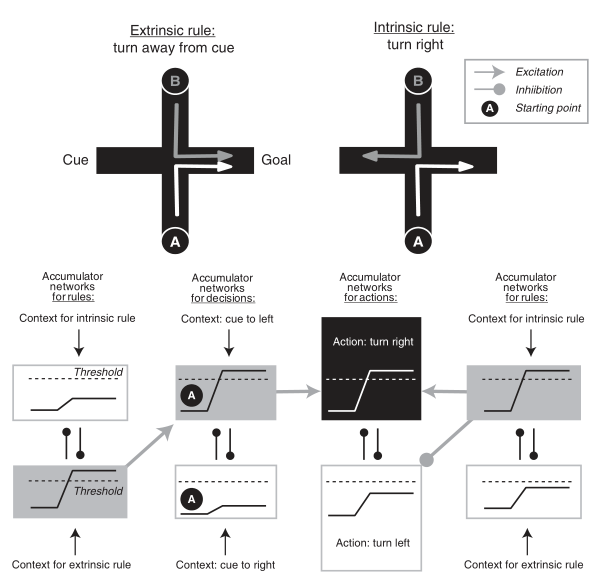
\includegraphics{image_pfc/Fig_3_6}
	\caption{基于外在规则与内在规则的选择的累加器网络模型。顶部:大鼠在加号迷宫的A点或B点开始每次试验。
		对于外在规则,他们需要选择一个与视觉线索相对的目标,在这个例子中是东方。
		对于内在规则,老鼠需要在选择点右转。底部:累加器网络如何导致两个规则(灰色背景)的右转(黑色背景)的概念描述。
		例如,当编码外在规则(左下角)的累加器网络达到阈值时,它们的输出抑制编码内在规则(左上角)的网络,并促进编码提示向左的感觉证据的网络,假设大鼠在A点开始试验。
		这些网络反过来为在这种情况下编码右转的网络提供证据。
		相反,对于内在规则,不同的网络(右上角)首先达到阈值,并促进右转,同时抑制左转。
		关键字:带圆圈的字母表示可能的起点。}
	\label{fig:3_6}
\end{figure}


Ragozzino等人\cite{ragozzino1999involvement}的一项实验使用了带有气味线索的加号迷宫。
在训练老鼠使用一条规则后,Ragozzino等人训练它们使用另一条规则。
这种新的学习涉及抑制或超越已经成为习惯的规则。
边缘前皮质和边缘下皮质的失活并没有损害大鼠学习初始规则的能力,无论是先学习的规则。但病变确实削弱了转换到第二条规则的能力。
确认所涉及的关键因素在两种规则之间切换,而不是一般的切换反应,Ragozzino\cite{ragozzino2007contribution}测试了大鼠在两种气味的选择之间的切换,大鼠表现正常\par


Rich\cite{rich2007prelimbic}使用视觉迷宫外线索扩展了这些结果。
边缘前皮质和边缘下皮质的失活导致内在规则和外在规则之间的切换受损,但不会影响大鼠在这两种规则中逆转其选择的能力。
重要的是,在规则切换当天,失活并没有影响性能。
相反,在第二天进行的测试中,病变导致了旧规则的使用增加和不正确。\par


Rich\cite{rich2009rat}还记录了规则转换过程中边缘前和边缘下皮层的神经元活动。
他们发现,边缘前皮质的活动变化发生得比边缘下皮质早。
当觅食选择在规则改变后有所改善时,边缘下皮层的活动就会发生变化。
这一发现可能反映了边缘前皮层提供的对结果导向行为的偏见,而边缘下皮层提供的是对习惯行为的偏见。
一般来说,这些区域中的细胞编码内在规则和外在规则之间的切换,但不编码规则内的切换。\par


这些结果表明,边缘前和边缘下皮层在指导基于竞争坐标系的觅食规则的变化。
当大鼠试图学习第二条规则时,它们必须使用结果导向的行为来做到这一点,并且它们需要它们的前大脑皮层来产生适当的偏见。
如果没有这种偏见,第一条规则中的习惯会干扰第二条规则的学习。
如果这第二条觅食规则在很长一段时间内保持有效,老鼠最终会将这条规则作为一种新的习惯。
图\ref{fig:3_6}显示了累加器网络如何实现这些规则,第 \ref{chap:chap6}- \ref{chap:chap8} 章更详细地介绍了前额叶皮层在学习和应用规则中的作用。\par


到目前为止,讨论的重点是内侧前额叶皮层的边缘前和边缘下部分。
下一节研究其剩余的无核成分,即前扣带皮层的作用。\par



\subsection{利益与成本之间的竞争}

当面临两种行动之间的选择时,动物不仅必须考虑到它们的相对利益,还必须考虑它们的相对成本。
在实验室里,实验者可以让动物在以大成本获得的大奖励和以小成本获得的小奖励之间做出选择。
作为成本的一个例子,实验者可以要求老鼠爬过障碍物以获得奖励\cite{salamone1997behavioral},或者在获得奖励之前等待\cite{cardinal2001impulsive}。
第一种操作带来了能源成本;第二种情况会带来延迟成本。\par


Walton等人\cite{walton2003functional}使用这些操作中的第一种对具有内侧前额叶皮层损伤的大鼠进行了测试。
在T型迷宫中,老鼠必须在两只手臂之间做出选择。
在一只手臂的末端,老鼠可以获得巨大的奖励,但它们只有爬过一道困难的屏障才能达到;
在另一只手臂的末端,他们可以获得少量奖励,而无需付出克服障碍所需的努力。
正常大鼠选择了两种奖励中较大的一种,尽管它们必须爬上相当大的障碍才能到达在这些条件下,前扣带皮层选择了较小的奖励(图\ref{fig:3_7})。
诱导老鼠爬上屏障需要相当大的奖励量的增加\cite{walton2002role}。\par


\begin{figure}[!htb]
	\centering
	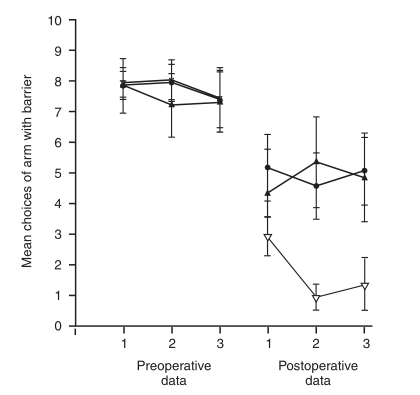
\includegraphics{image_pfc/Fig_3_7}
	\caption{努力成本对大鼠目标选择的影响。
		三组老鼠在迷宫的两臂之间进行选择。
		一只手臂有少量奖励,没有障碍物;另一只获得了巨大的奖励,并且有一个30厘米高的障碍,老鼠需要克服这个障碍。
		纵坐标显示了大鼠在10次试验中选择高强度手臂的平均次数。术后,前扣带皮层病变(未填充三角形)的大鼠选择高强度杆的频率明显低于其他两组:假病变(填充圆形)的大白鼠和边缘前加边缘下皮层病变(填充三角形)。
		误差条:SEM。横坐标上的1、2和3显示了3天的测试数据,每个测试10次。转载自Walton ME、Bannerman DM、Alterescu K、Rushworth MF。前扣带内侧额叶皮层内评估努力相关决策的功能专门化,《神经科学杂志》23:6475-9©神经科学学会,2003年,经许可。}
	\label{fig:3_7}
\end{figure}


Rudebeck等人\cite{rudebeck2006separate}比较了操纵成本在努力或延迟方面的影响。
大鼠前扣带皮层的损伤破坏了基于努力的选择,而眶额前额叶皮层的损伤则导致了基于延迟获得奖励的选择受损。
因为这项研究涉及大鼠,我们知道病变涉及颗粒缺失区域。
在下一章中,我们将研究眶额皮层这些部分的结果,但目前我们可以得出结论,无核前额叶皮层的内侧部分和眼眶部分都考虑了有关成本和收益的证据,并对所涉及的成本类型进行了一些专门化。
我们不知道同样的结论是否适用于猴子,但我们认为它们适用。\par


当一种行为不涉及觅食选择时,前扣带损伤不会损害依赖于努力成本的行为。
需要Schweimer\cite{schweimer2005involvement}大鼠越来越频繁地按下酒吧来获取食物,而前扣带回损伤并没有影响这种行为。
如果病变只是让大鼠变得懒惰或冷漠,那么当它们需要进行多次压条来生产食物时,它们就会停止压条。
Walton等人\cite{walton2002role}和Schweimer\cite{schweimer2005involvement}的实验不同之处在于,在前一种情况下,大鼠必须在两种动作之间做出选择,但在后一种情况中,它们没有。
沃尔顿等人的实验结果表明,当受损大鼠不得不根据预测结果做出觅食选择时,它们高估了努力成本或低估了回报收益。\par



\subsection{总结}

综上所述,我们利用啮齿类动物的证据证明,内侧前额叶皮层的无核部分的功能如下:\par


1.它们偏向于系统发育上较老的行为控制系统之间的竞争,以加快觅食选择的适应性。\par


2.它们将觅食选择偏向于适合稳定资源环境的习惯,或偏向于适合中等资源波动条件的结果导向行为。\par


3.它们在外在规则和内在规则之间进行导航选择,以指导觅食选择。\par


4.当动物必须根据预测结果的价值(包括努力成本)在行动之间做出选择时,它们在成本效益分析中发挥着至关重要的作用。\par


在这篇选择性综述中,我们强调了一个结果在奖励方面的当前生物学价值。
当然,对结果的评估更广泛地涵盖了其他类型的成本,如捕食或其他形式的伤害的威胁,以及其他类型的利益,如社会利益。\par


内侧前额叶皮层的连接决定了它如何执行这些功能。
投射到海马体、杏仁核、基底神经节和下丘脑和中脑导水管周围灰质的自主神经控制核可能传达了其自上而下的偏向。
来自海马体的输入提供了关于外在坐标系中导航的信息,而来自杏仁核的输入则提供了关于预测结果的当前值的信息。\par



\section{灵长类动物的无核皮层}

在上一节中,证据完全来自作为代表性啮齿类动物的老鼠,也许更有争议的是,作为代表性哺乳动物的老鼠。
正如第 \ref{chap:chap1} 章和第 \ref{chap:chap2} 章所解释的,大鼠的所有内侧前额叶皮层都具有颗粒缺失的细胞结构,就像其他哺乳动物一样。
在猕猴中,前扣带回皮层(24区)和边缘下皮层(25区)是无核的,而前边缘皮层(32区)的范围从无核到无颗粒\cite{Vogt&Derbyshire,2009;Mackey&Petrides,2010}。
猴子25区的亚属位置、细胞结构及其连接\cite{freedman2000subcortical}支持其被指定为大鼠边缘下皮层的同源物,以及类似的证据支持这样一个结论,即啮齿类动物和灵长类动物的前扣带回、边缘下皮层和边缘前皮层是同源的(第 \ref{chap:chap2} 章)。\par



\subsection{动作反转}

一项关键的实验评估了患有内侧前额叶皮层病变的猴子在动作之间切换的能力\cite{kennerley2006optimal}。
在动作反转任务中,猴子要在动作中做出选择。首先,他们学会执行一个动作,例如,在整个试验过程中始终如一地举起手柄。
之后,他们必须学会执行另一个动作,例如,在整个试验过程中始终如一地转动手柄。接下来是一系列进一步的反转。
对于每一次逆转,猴子都需要改变自己的动作选择,以产生奖励。
偶然性一词通常用来指一项行动与其结果之间的关系。
在动作反转任务中,猴子对同一个对象(手柄)执行两个不同的动作。
因此,没有任何外部线索促使做出适当的选择。
尽管如此,我们注意到猴子在物体上执行动作。\par
Kennerley等人在前扣带皮层(24区)造成损伤,包括头侧扣带运动区(CMAr)。
他们发现,扣带沟皮层受损的猴子在这两种动作之间的切换速度比正常猴子慢(图\ref{fig:3_8})\par


\begin{figure}[!htb]
	\centering
 	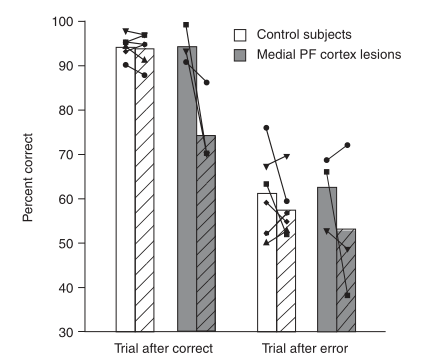
\includegraphics{image_pfc/Fig_3_8}
	\caption{行动选择的转回减值。
		猕猴的术前(实心条)和术后(孵化条)数据。
		对于正常(对照)猴子(白色)和受损猴子(灰色),正确选择后(左侧四条)和错误选择后(右侧四条)的正确百分比。
		猴子个体的结果用符号表示,并用线条连接。
		内侧前额叶皮层病变涉及前扣带沟的皮层,从沟的吻端到中央前沟的吻顶水平。
		请注意,受损伤的猴子在正确试验后做出的选择上有更大、更一致的损伤。
		经麦克米伦出版社有限公司Kennerley SW、Walton ME、Behrens TEJ、Buckley MJ、Matthew F、Rushworth S.的许可转载。最佳决策和前扣带皮层。《自然神经科学》9:940–7,©2006自然出版集团。}
	\label{fig:3_8}
\end{figure}


重要的是,这种损伤并不是由于坚持之前的行动造成的。
在一个关键的方法学进展中,Kennerley等人逐个试验分析了他们猴子的行为试验,而不是像心理学家传统上那样对一组试验进行平均。
这一过程使他们能够观察到,动物在通过奖励提供的正反馈和缺乏奖励提供的负反馈来指导他们的行动方面表现出低效。
对赤字的持续解释预测,使用负反馈的问题应该比使用正反馈的问题发挥更大的作用。
结果并没有证实这一预测。
事实上,这种损伤可以被描述为严重缺乏持久性:
与持久性相反。
与对照动物相比,那些有前扣带损伤的动物在正确的选择下坚持的时间更少,即使在五次以上的奖励后也是如此。
因此,猴子的前扣带皮层似乎促进了基于正反馈的有益选择的持续性,尤其是在行动发生变化后——结果偶然性促使猴子改变行动选择。\par


Behrens等人\cite{behrens2007learning}认为,这类任务的最佳策略取决于逆转的频率,这与自然觅食中资源可用性的“波动性”有关。
我们之前说过,大鼠的前大脑皮层会对行为产生偏见,这在中等波动的情况下是有利的。
例如,如果给定的条件在许多试验中占上风,那么很有可能会得到奖励,因为一次失败而立即切换到新的策略是不值得的。\par


Behrens等人扫描了受试者,同时他们在蓝色或绿色正方形的选择之间切换,这两者都与特定的概率和奖励幅度有关。
因此,这个实验涉及到在刺激之间的选择,而不是在动作之间的选择。
尽管如此,它还是导致了内侧前额叶皮层的激活,这是我们稍后重新讨论的问题。
Behrens等人寻找一种与受试者评估资源波动性的计算模型相结合的激活。
该模型是贝叶斯的,这意味着它使用关于概率的先验知识来评估关于世界的假设。
当给定某个事件时,如果假设为真,则该事件很可能发生,但如果假设为假,则不太可能发生,贝叶斯推理支持该假设。
在Behrens等人的实验中,由于奖励的波动性,受试者的假设变得错误。
Behrens等人在前扣带皮层发现了与选择相关的激活。
峰值激活发生在扣带沟和上覆的前SMA。
然而,与监测结果波动性相关的激活发生在内侧前额叶皮层,特别是在孕前脊髓前皮层(32区)。\par


Behrens等人研究对象之间的选择,而Kennerley等人研究行为之间的选择。
Rudebeck等人\cite{rudebeck2008frontal}特别比较了前额叶皮层损伤对学习对象-结果和行动-结果关联的影响。
他们在眶额前额叶皮层和内侧前额叶皮层(更具体地说,扣带回银行的前扣带回皮层)都有损伤。
第 \ref{chap:chap4} 章介绍了眶额皮层,我们比较了眼眶和内侧前额叶皮层。现在我们关注的是内侧前额叶皮层。
Rudebeck等人发现,前扣带皮层的损伤导致了基于行动的学习的缺陷,而不是基于对象的学习。因此,他们的数据支持这样一个结论,即猴子的内侧前额叶皮层在基于行动-结果关联选择行动方面发挥着重要作用。\par
Glascher等人\cite{glascher2009determining}使用成像来支持人类受试者的相同结论。
受试者被要求以两种方式之一移动电脑鼠标。当受试者在两个动作之间切换时,前扣带皮层发生激活。\par
本章是关于内侧前额叶皮层的,但我们知道它在真空中是不起作用的。在灵长类动物中,它似乎与位于其尾部的内侧前运动区密切合作,如前SMA和SMA。
与前扣带皮层的病变一样\cite{kennerley2006optimal},前SMA和SMA的病变会导致动作逆转任务的缺陷\cite{chen1995functions}。
在一项涉及行动和结果之间关联的不同任务中,Thaler等人\cite{thaler1995functions}表明,患有前扣带皮层或前SMA和SMA损伤的猴子(一起)在向上伸展以破坏不可见的红外光束方面表现出损伤。
在这个简单的任务中,结果的内部表示(一颗花生)作为动作的提示,猴子在完全黑暗的情况下进行了动作。
因此,前扣带和前运动皮层的损伤都会导致“内部”引导动作的损伤。
这种相似性表明,内侧前额叶皮层的颗粒缺失部分通过与内侧前运动区的连接影响动作的选择。\par



\subsection{价值的体现}
猴子的神经生理学研究表明,内侧前额叶皮层中的细胞编码各种结果变量。 Kennerley 等人\cite{kennerley2009evaluating}记录了内侧和眶额皮层细胞的活动。
在他们的任务中,猴子学习了类似物体的视觉刺激与奖励概率、奖励幅度或获得奖励所需的按键次数之间的映射。
然后猴子在两种刺激之间做出选择,它们几乎总是选择与更高收益或更低成本相关的刺激。
作者对内侧前额叶皮层和眶额皮层以及其他区域的细胞活动进行了采样,以寻找活动率与三个估值变量中的一个或多个的相关性。\par
根据前面提到的损伤结果,Kennerley等人预计眶额皮层将最显著地编码刺激-结果关联,而内侧前额叶皮层由于其与动作-结果关联的关系,对努力参数的编码更为稳健。
正如预期的那样,眶额皮层中的细胞编码刺激-结果估值(第\ref{chap:chap4}章)。
但内侧前额叶皮层的细胞也表现出这种活动,包括与所有三个决策变量相关的活动:奖励的大小、奖励的概率和获得奖励所需的按键次数。
对前扣带皮层(24区)的其他研究也发现了类似的结果相关信\cite{seo2007temporal,hayden2010neurons}。
回想一下,在Behrens等人\cite{behrens2007learning}的成像实验中,内侧前额叶皮层的激活反映了刺激之间的选择。\par
我们可以从几个方面来解释这些发现。从一个角度来看,他们同意与内侧前额叶皮层的行动-结果关联的归因。正如预期的那样,与分析努力成本相关的活动发生在内侧前额叶皮层。正如前面所述,人们也可以从决策、选择和行动的角度来解释这些结果。回想一下,从这个意义上说,决策反映了感官世界,而不是原始87种选择或行动中的AGRANULAL CORTEX\cite{schall1991neuronal}。
使用这个术语,我们可以建议内侧前额叶皮层将决策直接映射到行动,而眶额皮层通过物体之间的选择将决策间接映射到行动。
我们在第\ref{chap:chap4}章中再次讨论这个问题。\par
为了更全面地理解神经生理学的发现,我们想知道这些数据是来自内侧前额叶皮层的颗粒部分还是无颗粒部分。
Kennerley等人\cite{kennerley2006optimal}的研究中,损伤从扣带沟的头端延伸到几乎尾侧的4/6区边界(见图\ref{fig:1_2})。
因此,我们不知道该损伤的哪一部分导致了行动-结果学习的损伤。
如果没有这些知识,我们就无法从细胞结构的角度确定关键区域。
神经生理学数据可能会有所帮助,但不幸的是,无论是Kennerley等人\cite{kennerley2009evaluating}还是其他报告了类似结果的研究人员\cite{seo2007temporal,hayden2011neuronal}已经描述了它们的记录位点的细胞结构。\par


然而,Kennerley等人确实显示,在他们记录区的尾部,即胼胝体膝尾的扣带沟背岸,数值编码突然下降。
这种价值编码的下降对应于行动编码的增加。
Hayden等人还发现了对胼胝体膝部的吻侧编码的值。
人们很容易认为,它们记录区的嘴侧半部分对应于9区(颗粒皮层),尤其是扣带沟的背侧。
但Carmichael和Price的地图(图\ref{fig:fig_2_1}B)将该区域指定为猴子24区的一部分,因此我们在这里将其视为无核皮层。
在人类受试者中,有价值的扣带激活似乎在头端延伸到被称为32ac区\cite{Öngür et al. 2003}、32´区(Vogt 2009)或3簇\cite{Beckmann et al 2009}的区域。\par


除了编码结果的价值外,前扣带皮层的细胞还编码预期结果和发生的结果之间的差异。
在第\ref{chap:chap8}章中,我们讨论了奖励预测误差信号,它可能导致行为的强化和灭绝,这取决于差异的符号。
相比之下,前扣带皮层的错误信号在低估和高估结果方面没有差异\cite{Hayden et al,2011a}。
这个无符号错误信号只表明结果没有如预期的那样发生,并且行为上的一些调整是有序的。
这几乎没有表明这种调整应该是什么。
然而,这种神经信号反映了在监测结果中的作用,它可能有助于在坚持给定的行动方案和转向某种替代方案之间做出选择。\par


Hayden等人\cite{hayden2011neuronal}的一项细胞记录研究为这一想法提供了支持。
我们已经提到了这项开创性的研究。
它包含了本章的两个核心因素:灵长类动物在野外面临的觅食决策和前面解释的累加器网络。
海登等人发现了编码从不断减少的资源转换到新资源的价值的细胞。
每当猴子不得不在利用当前但正在减少的资源和转向新的资源之间做出选择时,前扣带皮层的细胞就会增加它们的活动。
猴子还收到了一个视觉信号,告诉它们开始开发新资源需要多长时间。
例如,比作从一块食物到另一块食物所需的时间,正如累加器-赛道模型预测的那样,每个延迟间隔,活动都向一个固定的阈值攀升,该阈值与切换到新资源的选择相关。
更长的延迟增加了这一阈值,从而实现了在许多动物中观察到的延迟折扣功能。\par


正如Kennerley等人和其他人的研究一样\cite{matsumoto2003neuronal,seo2007temporal},Hayden等人在前扣带皮层中观察到许多编码奖励价值的细胞\cite{hayden2009fictive,hayden2010neurons}。
这一结果似乎与实施留班选择的角色不一致。为了调和这两个发现,Hayden等人\cite{hayden2011neuronal}提出,在所有这些研究中,扣带皮层细胞编码了猴子利用有关资源的新信息做出选择的可能性。
在所有情况下,这种选择都涉及从持续开发资源到探索新资源的转变。\par


同样,Quilodran等人\cite{quilodran2008behavioral}表明,前扣带皮层的细胞编码在探索和开发阶段之间切换所需的反馈。
这种活动标志着探索期结束时的第一次奖励,而这些细胞在开发期停止编码奖励。在新的探索期开始时,活动又恢复了。\par


一项针对人类受试者的成像研究支持这样一种观点,即前扣带皮层监测结果,以选择有利的动作。
Walton等人\cite{walton2004interactions}表明,当受试者做出自己的动作选择时,背侧前扣带皮层的激活会增加,但当实验者选择动作时,同一区域的激活会减少。
因此,前扣带皮层似乎在监测自我产生的行为中发挥着作用,这一想法我们稍后在讨论额极皮层时会回到。
同样的研究人员还表明,当结果提供反馈信息时,无论结果是阳性还是阴性,前扣带回皮层都会发生激活。
在之前的研究中,建议在错误监测中发挥作用,只有错误才能提供反馈\cite{yeung2004neural}。
Walton等人的研究结果表明,内侧前额叶皮层的功能比错误检测或冲突解决更为普遍。\par



\subsection{啮齿类动物和灵长类动物的比较}

第\ref{chap:chap2}章解释了大鼠缺乏颗粒状前额叶皮层的同源物。
因此,我们看到灵长类动物的内侧前额叶皮层的无核部分与啮齿类动物的整个内侧前额叶皮层相对应。
因此,我们在前两个主要部分中讨论了啮齿类和灵长类动物的无核前额叶皮层。
然而,其他人对此事的看法不同。当他们的观点与内侧前额叶皮层直接相关时,我们在这里简要地提到他们。
稍后,第\ref{chap:chap10}章更全面地讨论了物种比较的问题。\par


Uylings等人\cite{uylings2003rats}以及Seamans\cite{seamans2008comparing}提出,大鼠的内侧前额叶皮层与中外侧前额叶皮层(区域46)同源,尽管前者具有无颗粒细胞结构,而后者具有颗粒结构。
为了支持他们的结论,他们认为大鼠的内侧前额叶皮层与猴子的颗粒状前额叶皮层有许多相同的财产,其中他们包括空间记忆任务损伤后的损伤和细胞活动的一些财产。\par


但这些财产并没有说明同源性,因为它们广泛应用于额叶皮层,包括颗粒和无颗粒区域。
第\ref{chap:chap2}章解释了诊断特征将一个区域与其他区域区分开来,这些特征越多,结论就越有力。
所有相关领域的共同特征没有提供关于同源性的指导。
因此,无论是损伤效应还是其他财产都不支持啮齿类动物内侧前额叶皮层与灵长类动物颗粒状前额叶皮层的任何部分的同源性。\par


我们知道,内侧前额叶皮层的损伤会对大鼠的延迟反应任务造成损害\cite{kolb1974double}。
但猴子的前扣带皮层和前边缘皮层的损伤也是如此\cite{meunier1997effects},类似的损伤会导致延迟交替任务的损伤\cite{rushworth2003effect}。
鉴于这些发现,大鼠的损伤没有提供诊断证据表明大鼠的内侧前额叶皮层与猴子的中外侧前额叶皮层同源。\par


大鼠和猴子的损伤可能对类比有一些影响,而不是同源性\cite{brown2002rodent}。
然而,空间信息处理包含了广泛的功能,包括导航、到达、地点识别、距离识别等。
人们不得不争辩说,一项任务是对其中一种功能的纯粹测试,以便为大鼠的内侧前额叶皮层和猴子的中外侧前额叶皮层之间的类比提供令人信服的理由。
目前还没有人提出这样一个有效的论点。\par



\subsection{总结}

在大鼠和猴子中,颗粒状内侧前额叶皮层似乎在根据预测结果选择行动方面发挥作用。
基于行动和结果之间的联系,动物可以选择特定的行动。
他们还可以选择继续做他们一直在做的事情,或者换做其他事情。
内侧前额叶皮层有助于两种选择。
因此,它不仅仅是将行动与结果联系起来,以影响采取特定行动的频率、付出多少努力,或者根据对奖励幅度或概率的预期采取何种行动。
它执行这些功能,但除此之外,它还有助于选择抽象操作(利用或探索)或特定操作。
它在内部或外部坐标中这样做。
后者发生在动物选择一个地方作为行动目标时; 前者发生在他们直接选择一个动作时。
当结果可靠地满足预期时,内侧前额叶皮层的某些部分会使行为偏向于不考虑预测结果(习惯)的行为;
当结果不太符合预期时,内侧前额叶皮层的其他部分会将行为偏向基于预测结果的行为。\par



\section{颗粒皮质}

如果我们接受这些结论,我们仍然需要说明猴子内侧前额叶皮层的颗粒部分与其无颗粒部分有何不同。
区域10对应于额极皮层并且区域9的内侧部分对应于背内侧前额叶皮层。
两者都有颗粒状的细胞结构,第\ref{chap:chap2}章回顾了它们在类人猿灵长类动物中进化的证据。
请注意,我们将前扣带皮层一词保留为无颗粒区域,因此到目前为止,我们所说的前扣带皮质都不是指这两个颗粒区域中的任何一个。\par


首先,我们承认数据匮乏。
除了在人类受试者中的成像发现外,很少有实验涉及灵长类动物9区或10区内侧部分的功能。
查阅大鼠文献并没有提供任何指导,因为正如第\ref{chap:chap2}章所解释的,大鼠缺乏这些颗粒状前额叶皮层的任何同源物。
因此,本章的其余部分所依赖的数据比我们希望的要少。\par


和往常一样,我们从连接解剖学中寻找线索。
在此基础上,我们认为内侧颗粒区阐述了内侧前额叶皮层颗粒缺失部分的功能。
正如前面关于连接的部分所解释的,所有内侧区域主要接受“内部”输入,而外部输入很少。
我们认为,当可用的外部线索不表明要采取什么行动时,它们都会产生行动或行动规则的选择,并使其产生偏见。
在这种情况下,行动的选择取决于在没有外部提示的情况下预测结果的值。
我们认为内侧前额叶皮层的颗粒部分扩展了这些功能。\par



\subsection{任务规则}

Desmet等人\cite{desmet2011errors}的一项研究有助于阐明内侧前额叶皮层的头侧和尾侧部分之间的区别。
当奖励反馈告知人类受试者应该做出什么动作时,激活发生在内侧前额叶皮层的尾部,即前扣带皮层。
当奖励反馈告知受试者要执行哪项任务,而不是要采取什么具体行动时,内侧前额叶皮层的一个更为突出的部分被激活。
Venkatraman等人\cite{venkatraman2009resolving}获得了类似的结果。
这些发现表明,内侧前额叶皮层的嘴侧部分有助于在两项任务之间做出选择,并且它们通过内侧前额叶皮层更多的尾侧部分影响特定的动作。\par


在猴子身上,当猴子需要解决两种规则之间的冲突时,额极皮层(10区)的损伤会导致任务表现的改善(M.J.Buckley,个人交流)。
此外,受损的猴子,而不是正常的猴子,在参与第二项任务或在试验之间提供意外奖励后,成功地回到了正在进行的主要任务。
就像刚才提到的成像结果一样,这些发现指出了最具头侧前额叶皮层在影响两种任务规则之间的偏差方面的作用。
第\ref{chap:chap9}章针对人类主题展开讨论。\par



\subsection{自我生成的目标}

猴子内侧 9 的唯一神经生理学发现来自Tsujimoto等人\cite{tsujimoto2006direct}的一项研究。
这些研究人员测量了中间区域9和32的θ振荡。
Theta波是频率为4–7赫兹的电势。
Tsujimoto等人报告了三个发现:
(1)在猴子进行自我启动运动之前发生的θ振荡的功率增加;
(2) 在th的功率也有类似的增长奖励时间;
以及(3)两个区域之间的振荡相干性。
Theta振荡可以组织皮层中表示的信息,关于奖励前后自我生成目标的发现预示着接下来从额极皮层(区域10)解释的那些目标。\par


\begin{figure}[!htb]
	\centering
	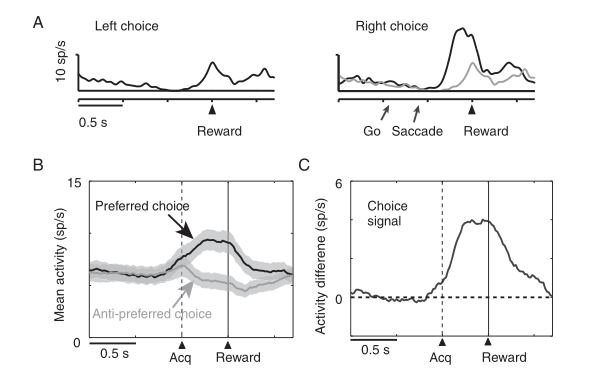
\includegraphics{image_pfc/Fig_3_9}
	\caption{额极皮层(区域10)中反馈时间的细胞活动编码选择。
		A) 奖励时编码向右目标选择的单元格中的活动(右)。左侧选择的活动在右侧的图中以灰色复制。(B) 每个细胞的首选(黑色)和备选(反首选)(灰色)的群体活动。缩写:acq,目标的获取。着色:扫描电镜。(C)选择信号表示为(B)中曲线之间的差异。数据来自Tsujimoto S,Genovesio A,Wise SP。评估猴子额叶皮层中自我生成的决策,《自然神经科学》13:120–126©2010。}
	\label{fig:3_9}
\end{figure}


另一位名叫Tsujimoto的神经科学家研究了额极皮层(10区)的神经元活动,而猴子则进行视觉提示策略任务\cite{tsujimoto2010evaluating}。
在每次试验中,一个提示指示猴子向与前一次试验相同的方向扫视(“跳跃”提示)或向相反的方向扫视。
如图\ref{fig:3_9}所示,Tsujimoto等人发现,额极皮层的神经元编码了猴子在每次正确执行的试验中选择的目标,并且它们只在反馈(结果)前后这样做。\par


注意,提示并没有直接指定扫视的方向或目标。
提示只是告诉动物坚持最近的成功目标,或者转向另一个目标。
猴子不得不用它对上一个目标的记忆来选择下一个目标。
换句话说,尽管停留和转移的线索是外部的,但猴子必须在内部信号的基础上产生目标。\par


在同一个实验中,Tsujimoto等人包括了一种条件,在这种条件下,空间线索指示动物在每次试验中选择哪个目标:动眼器延迟响应任务。
他们比较了在正常时间出现反馈时的活动与比正常时间晚的反馈活动。
在后一种情况下,神经元信号直到反馈到达才持续。
相比之下,在提示策略任务中,在所有情况下,在反馈之后,细胞继续对所选择的空间目标进行几百毫秒的编码。
Tsujimoto等人将这一发现解释为,与动眼神经延迟反应任务中纯粹由外部指示的目标相比,额极皮层在评估自我产生的目标方面发挥着重要作用。
所有目标编码都发生在结果出来的时候,这一发现表明,在正在进行的试验中,额极皮层在未来目标的选择中发挥作用,而不是在目标的选择上。\par


Tsujimoto等人还比较了错误试验和正确试验期间的活动。
他们假设,在正确的试验中,猴子根据提示策略(“停留”或“转移”)产生了一个目标,而在错误试验中,猴则在其他基础上产生了目标。
与正确试验中的稳健目标编码相反,相同的神经元在错误试验中几乎没有编码目标,如果他们真的这样做的话。
这一发现表明,额极皮层编码基于提示策略产生的目标,这需要外部提示和对最近先前目标的记忆的结合。
当猴子在其他基础上选择目标时,额极皮层对目标的编码很弱(如果有的话)。\par


在下一章中,我们建议颗粒状前额叶皮层允许猴子将单个事件与结果联系起来,并将这种学习与许多试验中对关联的缓慢调整进行对比。
所选目标在结果发生时的表现可能有助于学习这些联系。\par



\subsection{单个事件}

其他证据也表明了单一反馈事件的重要性。
Gaffan\cite{gaffan1992amnesia}设计的一项任务,称为物体原位场景任务,允许对基于事件的学习进行研究。猴子看到一系列彩色、复杂的背景场景,每个场景都包含两个彩色形状(字母),它们总是出现在特定场景的同一位置。
猴子需要学会选择哪种颜色的形状才能获得奖励。\par


猴子学习这项任务的速度非常快,即使它们在任何场景重复之前都会看到一系列20个场景。
这种快速学习可能取决于猴子将触摸特定颜色形状的记忆嵌入由特定背景场景组成的特定上下文中的能力。
目标(彩色形状)、动作(触摸它)、背景(背景场景)和结果(奖励)的结合构成了一个事件。\par


Piekema等人(2009年)将这项任务交给了患有\textit{额极皮层}皮层病变(10区)的猴子。
这些损伤在每个场景的第二次呈现时都会造成严重的损伤,但此后猴子恢复了相当正常的学习速度(图\ref{fig:3_10})。
当然,对照猴子在第二次演示后的改进空间比受损猴子小。
因此,我们只能说,在第二次演讲后,学习率似乎大致相当。
关键是第二次演示对每个场景的记忆评估了猴子记忆单个事件的能力,这些事件包括它们对20个场景中的每个场景的初始选择,并从长期记忆中回忆它们。
第\ref{chap:chap8}章认为,这一发现在很大程度上解释了前额叶皮层。\par


\begin{figure}[!htb]
	\centering
	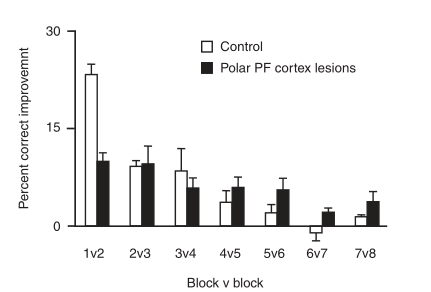
\includegraphics{image_pfc/Fig_3_10}
	\caption{额极皮层(区域10)损伤后,第二次试验的物体原位场景任务损伤。每个条形图显示了正常(对照)猴子(白色)和病变猴子(黑色)连续试验块的正确选择百分比的差异。
		每个选项在20个选项的“块”中出现一次。
		缩写:v,相对于。数据来自Piekema等人(2009年),由Mark J.Buckley博士提供。}
	\label{fig:3_10}
\end{figure}



\subsection{事件存储器}

在认知心理学中,情景记忆是指对单个事件的回忆。
对于猴子的研究,我们避免使用这个术语,因为它意味着对事件的认识。
然而,在人类身上,评估意识往往很容易。
实验人员可以简单地要求受试者回忆他们生活中的事件,称为自传体记忆。
因此,例如,Hassabis等人\cite{hassabis2007using}要求受试者记住他们做过的事情,比如在电影院的摊位上买票。
这些事件包括在特定时间和地点的行动、目标、背景和结果的结合。
Hassabis等人随后将受试者对这类行为的记忆与对物体的记忆进行了对比。
在内侧前额叶皮层(9区)、脾后皮层和海马体中,两种记忆(事件记忆和对象记忆)发生了不同的激活。
类似地,Summerfield等人\cite{summerfield2009decision}在受试者从情景记忆中检索不同类型的事件时对其进行了扫描。
他们在额极皮层的内侧部分(10区)、脾后皮层和海马体中发现了激活。\par



\subsection{总结}

具有额极皮层损伤(区域10)的猴子在物体原位场景任务的第二次试验中有损伤;
额极皮层中的细胞在反馈时编码自我生成的目标;
并且当人类受试者检索单个自传体事件的记忆时以及当他们在任务规则中进行选择时,在额极皮层(中间区域10)和中间区域9中具有激活。
对象就地场景任务可能反映出未能从长期内存中检索相关事件,或者未能使用该内存来影响当前的目标选择。
背景场景提供了当前的背景,第二次审判的正确选择取决于一次审判从单个自传体事件中学习。\par


早些时候,我们认为内侧前额叶皮层的无核部分会在动作或基于动作的规则之间产生偏差。
这些偏见取决于“内部”信号,这些信号涉及动机状态和对先前事件的记忆,包括行动和结果。
在本节中,我们提出内侧前额叶皮层的颗粒部分阐述了颗粒缺失部分的功能。两者都主要使用“内部”信号来指导选择。
有时,这些选择涉及对对象执行的动作,有时也涉及动作本身。
细粒度区域通过“内部”生成目标或规则,并通过实施一次尝试学习的机制,即基于单个事件的学习,来阐述非细粒度区域的功能。
其机制的一部分涉及在反馈时对所选目标的表示,以及随后从长期记忆中检索该事件。\par



\section{结论}

\subsection{内侧前额叶皮层如何发挥作用}

内侧前额叶皮层与海马体、杏仁核和内侧前运动区的连接解释了其对整个前额叶皮层的贡献:\par

1.内侧前额叶皮层通过脾后皮层、内嗅皮层和丘脑与海马系统有着强烈的相互联系,既有直接联系,也有间接联系。由于海马体在外部(非中心)坐标系中引导导航的作用,当海马体控制行为时,应该出现对外部引导规则的偏见。有证据表明,当基于内在指导的规则占主导地位时,基底神经节的部分控制行为\cite{packard1996inactivation}。
内侧前额叶皮层,特别是其边缘前和边缘下区域,提供了一种自上而下的偏向。
更普遍地说,这种自上而下的偏见提供了一种机制,通过这种机制,内侧前额叶皮层可以发挥注意力控制,在第\ref{chap:chap8}章中,我们认为前额叶皮层作为一个整体发挥这种控制。\par


与海马系统的连接也向内侧前额叶皮层提供了有关导航和其他动作相关事件的信息,在第\ref{chap:chap9}章中,关于人类前额叶皮层,我们提出导航和事件信息有助于将自己的动作嵌入事件的表现中。\par


2.内侧前额叶区域与杏仁核的联系解释了这些区域如何将行动与结果的当前价值联系起来。当动物消耗液体或营养物质时,它们的需求会发生变化,杏仁核和前额叶皮层之间的相互作用会更新对涉及这些资源的行为结果的评估。
类似的更新可能发生在负面结果上,如努力成本、行动的有害结果和引发恐惧的刺激。这些评估对与这些结果相关的行动之间的选择产生了偏见。\par


当期望值未能实现时,动物需要改变它们的行动,而内侧前额叶皮层促进有效利用奖励反馈来执行这种行动逆转,包括在利用日益减少的资源和让它去探索新的资源之间进行切换。\par


3.与内侧运动前区的连接允许内侧前额叶皮层影响运动命令。\par

尽管这三组连接往往集中在内侧前额叶皮层的尾部无核部分,但无核区和颗粒区之间的牢固连接使内侧前额叶皮层作为一个整体能够使用它们。
第\ref{chap:chap9}章讨论了人类内侧前额叶皮层的层次结构(见图9.7)。\par



\subsection{目的}

在第\ref{chap:chap8}章中,我们提出了一个关于前额叶皮层整体基本功能的建议。
每个区域都有助于实现这一功能,因此我们以一份关于内侧前额叶皮层的声明开始制定我们的提案,首先是最简短的形式,然后是扩展版本。\par


简而言之:\par
内侧前额叶皮层有助于根据与结果的关联,根据当前需求,在行动中进行评估和选择。\par
扩展:\par
内侧前额叶皮层通过对基于动作的动作和规则之间的选择产生偏见,对整个前额叶皮层的功能做出贡献。
它通过根据当前需求评估预期结果来做到这一点。
当结果不能满足当前需求时,内侧前额叶皮层会促进有效利用这种反馈,在利用日益减少的资源和探索新的资源之间切换,在替代行动之间切换、在竞争行动规则之间切换,以及在竞争行为控制系统之间切换。
在灵长类动物中,它可以基于单个事件来做到这一点。\par



\subsection{为什么其他区域不能像内侧前额叶皮层那样}

其他区域不能做内侧前额叶皮层所做的事情,因为它们缺乏一个或多个关键连接。
前额叶皮层的许多其他部分缺乏海马连接。
后顶叶皮层与皮层的运动前区域有直接联系,如内侧前额叶皮层,但至少在任何明显的程度上缺乏杏仁核的联系(图\ref{fig:3_3})。
同样的限制也适用于大脑皮层的许多其他部分。
颞上皮层和颞下皮层与杏仁核有联系——视觉区域更是如此——但与内侧前额叶皮层的运动前区域缺乏直接联系。\par



\subsection{对觅食选择的贡献}

内侧前额叶皮层帮助动物在竞争动作中做出选择。
在许多情况下,在选择时没有外部提示提示动物。
动物可以看到(或其他感觉)许多刺激,但没有一个提供选择一个动作而不是另一个动作的基础。
在这种情况下,只有一个动作与其结果的关联才能使动物在动作中做出选择。
在觅食过程中,动物通常需要在没有任何外部提示的情况下在潜在动作中进行选择。
当然,自然环境中有很多线索,但它们往往无法为该做什么提供指导。
在这种情况下,行动-结果映射提供了必要的指导。\par


内侧前额叶皮层的细胞根据数量、发生概率和努力成本对结果进行编码,所有这些因素都会进入觅食选择。
因此,无核内侧前额叶皮层会使竞争动作、竞争坐标系和不同类型的联想之间的竞争产生偏差,所有这些都可能在某些情况下导致成功。
例如,当由于资源波动性增加,习惯性觅食选择变得不那么有效时,内侧前额叶皮层的一部分会对结果导向行为产生偏见。
另一部分产生了相反的偏见,在稳定的觅食环境中促进快速、自动的行为。\par


内侧前额叶皮层的颗粒部分对类人猿的觅食选择做出了额外的贡献。
关于它们的功能,我们只有几条线索:
当人们回忆自传体事件或产生任务规则时,激活发生在9区的中部或额极皮层(10区);
猴子额极皮层中的细胞在反馈时间编码自我生成的目标;
额极皮层的损伤损害了猴子利用单个事件选择未来目标的能力。
这些发现指出了为目标分配结果的作用,以改善未来的选择\cite{tsujimoto2011frontal}。\par
事件的概念对这些结论很重要。我们所说的事件是指特定时间和地点的背景、目标选择、行动和结果的结合。
正如类人猿灵长类动物所面临的那样,根据先前的单一事件做出觅食选择可以为寻找高度波动的资源提供优势(第\ref{chap:chap2}章)。
第\ref{chap:chap4}章至第\ref{chap:chap7}章认为,单个事件在颗粒状前额叶皮层的功能中发挥着重要作用,第\ref{chap:chap8}章认为,利用单个事件选择目标的能力是前额叶皮层基本功能的核心。\par
本章回顾了内侧前额叶皮层根据其与价值结果的关联对选择行动做出贡献的证据。
动物可以通过在物体之间进行选择来直接或间接地选择动作。
我们认为,内侧前额叶皮层的连接使其能够在动作选择中发挥作用,尤其是当这些选择发生在没有告诉动物该做什么的外部感觉信号的情况下时。
下一章将讨论眶额皮层,它在物体选择中的作用,以及为什么内侧前额叶皮层和眶额皮层必须相互作用。\par



